\chapter{今後の課題とまとめ}
\label{chapter:conclusion}

本章では、本研究で提案したアクターシステムの検証ライブラリActarioの今後の課題と、本論文のまとめを述べる。

\section{今後の課題}

Actarioはアクターモデルの基本的な部分を実装、
そして本論文ではActarioを使って単純な例題の証明を示しただけに過ぎず、
実際のアクターアプリケーションの検証に耐えられるものであるとは言いづらい。
本節では実用に耐えられる検証ライブラリにするための今後の課題をいくつか述べる。

\subsection{証明が完了していない部分の証明}
第\ref{chapter:proof}章で述べた\coqi{trace_path}についてである。
この補題の直感的な理解は述べたが、アプリケーションの検証に使われることが多いこの補題がもし証明可能でないならば、
\coqi{trace_path}を検証に用いたアプリケーションの証明は崩れてしまう。

また、\coqi{trace_path}に関連して、公理となっている\coqi{path_perm}を\coqi{path}の述語として定義すべきである。
こうすべき理由も\coqi{trace_path}と同様に証明の一貫性を崩してしまう可能性があるからである。

\subsection{より複雑な例題の検証}
より複雑な例題、特に繰り返しの構造が入るようなものについて検証を試みる必要がある。
例えば、\ref{chapter:overview}で述べた階乗を計算するアクターシステムだと、図\ref{code:conclusion:fact-n}のような、任意の自然数に対して正しく階乗を計算するシステムであるといった命題などである。
証明の方法としては、以下の三つの補題に分け、それぞれについて証明する。

\begin{figure}[tp]
\begin{lstlisting}
Definition top := toplevel "factorial".
Theorem receive_n :
  forall n,
    eventually_receive (factorial_system n top)
                       top
                       (nat_msg (fact n)).
\end{lstlisting}
  \label{code:conclusion:fact-n}
  \caption{階乗計算システムが任意の自然数に対して正しく階乗を計算するという定理}
\end{figure}

%% これを証明するためには何らかの値に対して帰納法を使う必要があるが、単純に階乗を計算したい自然数$n$に対して帰納法を使うと、帰納法の仮定が\coqi{factorial_system k top}についてのパスに関する式、ゴールが\coqi{factorial_system (k + 1) top}についてのパスに関する式という形になり、帰納法の仮定が使えない。

\begin{enumerate}
\item 任意の自然数について、システム実行開始から図\ref{img:conclusion:fact}の\textcircled{\scriptsize 1}まで遷移する
\item 任意の自然数について、図\ref{img:conclusion:fact}の\textcircled{\scriptsize 1}から\textcircled{\scriptsize 2}まで遷移する
\item 任意の自然数について、図\ref{img:conclusion:fact}の\textcircled{\scriptsize 2}からトップレベルアクターが\textsc{Receive}遷移をする(\textcircled{\scriptsize 3})
\end{enumerate}

\begin{figure}[tp]
  \centering
  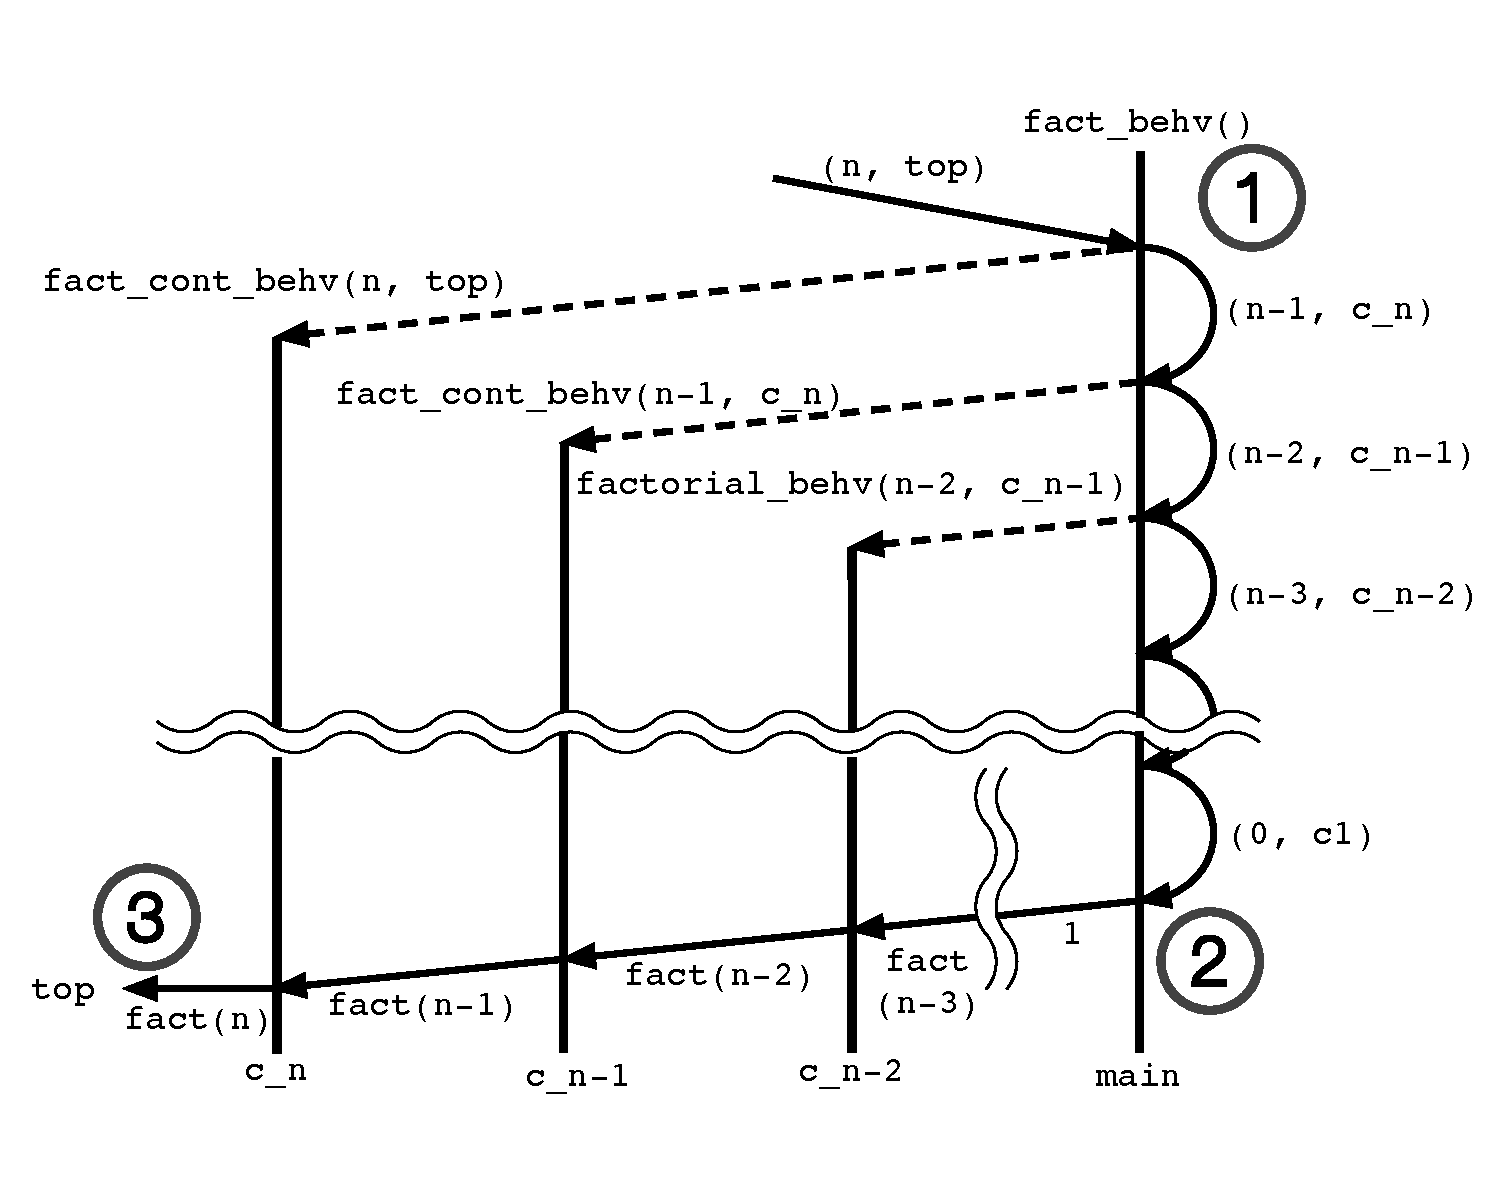
\includegraphics[width=16cm]{./img/conclusion/fact_n.pdf}
  \label{img:conclusion:fact}
  \caption{$n$の階乗を計算するシステムの動き}
\end{figure}

しかし、現在の証明機構では、ラベルおよびそのラベルによって遷移した後の配置を計算するために、配置内のすべてのアクターが具体的に定まっている必要がある。
このシステムでは配置内のアクターは自然数$n$によって決定するので、配置は具体的には定まらない。

また、配置を具体的に決定できなくても図\ref{code:conclusion:possible-labels-cat}の補題が成り立てば少し証明がやりやすくなるが、これは\textsc{Send}遷移の際に送り先の状態(メッセージキュー)を操作する必要があるため成り立たない。
\textsc{Send}遷移をする際に送り先のメッセージキューに直接メッセージ入れず、バッファとなるようなものを用意して一時的にその部分に保存するようにすれば、この問題は解決できるが、そのような実装にしたことで確かに具体的な配置がわからなくても証明ができるようになるか、また他の定理や証明機構に影響を及ぼさないかどうかは検証の余地がある。


\begin{figure}[tp]
\begin{lstlisting}
Lemma possible_labels_cat :
  forall c c',
    possible_labels (c ++ c') =
    possible_labels c ++ possible_labels c'
\end{lstlisting}
\label{code:conclusion:possible-labels-cat}
\caption{\coqi{possible_labels}についての補題}
\end{figure}


さらに、\fairness を用いなければ証明できないような命題の証明を行えるような仕組みを整えなければいけない。
例えば、図\ref{code:conclusion:pingpong}のような、1. pingというメッセージを受け取ると、pingメッセージの送り主に対してpongというメッセージを送信するサーバ、2. サーバに対してpingというメッセージを送り続ける2つのクライアント、を考える。このシステムは図\ref{code:conclusion:pingpong-spec}、つまりを満たすべきだが、
\ref{chapter:proof}で定義した\coqi{fairness}を使うためには、あるラベルが遷移可能になることが無限に繰り返されるようなパスであることを示す必要があり現状の証明機構では使いづらい。そのため、\coqi{fairness}を使いやすいようなタクティクなどの仕組みを作るか、\coqi{fairness}自体を同等または弱い性質でかつ扱いやすいものに定義し直す必要がある。

\begin{figure}[tp]
\begin{lstlisting}
(**
 * ping というメッセージを受け取ると、
 * pong というメッセージを送り主に送信する
 *)
Definition server_behavior (state : unit) : behavior unit :=
  receive (fun msg =>
         match msg with
           | tuple_msg (name_msg sender) (str_msg "ping") =>
             sender ! (str_msg "pong");
             become state
           | _ => become state
         end).

(* メッセージを受け取るとサーバに ping というメッセージを送る *)
Definition client_behavior (server_addr : name) : behavior name :=
  receive (fun _ =>
    me <- self;
    server_addr ! (tuple_msg (name_msg me) (str_msg "ping"));
    become server_addr
  ).

Definition pingpong_system : config :=
  init "pingpong" (
    server <- new server_behavior with tt; (* サーバーを作る *)
    (* クライアント1を作る *)
    client1 <- new client_behavior with server;
    (* クライアント2を作る *)
    client2 <- new client_behavior with server;
    client1 ! empty_msg; (* クライアント1を走らせる *)
    client2 ! empty_msg; (* クライアント1を走らせる *)
    become done (* それ以降は何もしない *)
  ).
\end{lstlisting}
  \label{code:conclusion:pingpong}
  \caption{ping-pongシステム}
\end{figure}

\begin{figure}[tp]
\begin{lstlisting}
Definition client1_name := generated 1 (toplevel "pingpong").
Theorem receive_client1 :
  eventually_receive pingpong_system
    (generated 1 top) (str_msg "pong").
\end{lstlisting}
  \label{code:conclusion:pingpong-spec}
  \caption{ping-pongシステムが満たすべき性質}
\end{figure}

\subsection{障害の形式化}
本ライブラリの最終目標としては、障害が起こりうる環境においてもシステムの性質は成り立つというような命題に対して検証を行えるというものだったが、それはまだ達成できていない。
これを達成するためには、まず障害を形式化し障害を含むような意味論にすること、障害から復旧させるような機構を導入すること、が挙げられる。

%% 障害を含むような意味論は図\ref{code:conclusion:failure}のようなものになると考えられる。

%% \begin{figure}
%% \label{code:conclusion:failure}
%% \caption{障害を含むような意味論}
%% \end{figure}

また、障害を含むような場合と障害を含まないような場合で分けて検証できるように、意味論を切り替えられるようにすることが必要である。
この手法はVerdiが行っているもので、こうすることによって、ある障害については耐性があるが、別のある障害に対しては耐性がない、というようなことも検証できるようになる。


\section{まとめ}

本論文では、アクターシステムの検証ライブラリActarioを提案した。
ActarioはまずActarioが提供する構文を用いてアクターシステムを記述し、その性質をActarioの補題とタクティクを使って検証、そしてErlangに抽出するというものである。これらを実例を見ながら説明した。
Actarioではアクターの名前はシステムによって暗黙的につけられるようになっており、またその名前付けの一意性はCoqにより形式的に証明されている。
アクターシステムの検証を簡単にするための機構、そして抽出の方法について説明した。

Actarioを使って検証したアクターシステムの例は簡単なものだけであり、またアクターシステムの検証のための補題やタクティクも少ないので、まだまだ実用的ではないと言わざるを得ない。
大規模で複雑なシステムの検証のため補題やタクティクを補強することが課題である。
